\documentclass[10pt,a4paper]{article}
\usepackage[usenames,dvipsnames]{xcolor}
\usepackage{tikz} % for drawing figures
\usepackage{amsmath} % for equations
\usepackage{url} % for URLs
\usepackage{graphicx}
\usepackage{multicol}
\usepackage{varwidth}
\usepackage{blindtext}
\usepackage{nicefrac}


\usepackage{linguex} % ** special include in directory: for doing handy example labeling and bracketing
\renewcommand{\firstrefdash}{} % used for linguex package not to put hyphens in example refs (1a instead of 1-a)
\usepackage{cogsci}
\usepackage{pslatex}
\usepackage{apacite}

\newcommand{\sem}[1]{\mbox{$[\![$#1$]\!]$}}
\newcommand{\lam}{$\lambda$}
\newcommand{\gcs}[1]{\textcolor{Blue}{[gcs: #1]}} 
\newcommand{\mf}[1]{\textcolor{BrickRed}{[mf: #1]}} 


\title{Subjectivity-based adjective ordering maximizes communicative success}
\author{\large \textbf{our names}\\
our emails\\
our affiliations}


\begin{document}
\maketitle

\begin{abstract}
Adjective ordering preferences (e.g., \emph{big blue box} vs.~\emph{blue big box}) are robustly attested in English and many unrelated languages \cite{dixon1982}. \citeA{scontrasetal2017adjectives} showed that adjective subjectivity is a robust predictor of ordering preferences in English: less subjective adjectives are preferred closer to the modified noun. In a follow-up to this empirical finding, \citeA{simonic2018} and \citeauthor{scontrasetalSPadjectives} (to appear) claim that pressures from successful reference resolution and the hierarchical structure of modification explain subjectivity-based ordering preferences. We provide further support for this claim using large-scale simulations of reference scenarios, together with an empirically-motivated adjective semantics. In the vast majority of cases, subjectivity-based adjective orderings yield a higher probability of successful reference resolution.


\textbf{Keywords:} 
adjective ordering, subjectivity, reference resolution, hierarchical modification

\end{abstract}

\section{Introduction}

When speakers use two or more adjectives to modify a noun, they exhibit robust preferences in the relative order of the adjectives (e.g., \emph{big blue box} vs.~\emph{blue big box}). These preferences surface also in listeners as they encounter multi-adjective strings. Using a series of behavioral and corpus experiments, \citeA{scontrasetal2017adjectives} demonstrated that adjective order in multi-adjective strings is reliably predicted by the subjectivity of the adjectives involved: less subjective adjectives are preferred closer to the modified noun, and the strength of the preference is modulated by the subjectivity differential between the adjectives. Thus, speakers and listeners strongly prefer \emph{big blue box} over \emph{blue big box}, as \emph{blue} is much less subjective than \emph{big}.

The question that immediately arises is why subjectivity should play the role it does in adjective ordering preferences. The current work follows \citeA{simonic2018} and \citeauthor{scontrasetalSPadjectives} (to appear) in advancing the claim that pressures from successful reference resolution deliver subjectivity-based ordering preferences. In cases of restrictive modification, adjectives that compose with the nominal later will classify a smaller set of potential referents (e.g., the set of boxes vs. the set of blue boxes). To avoid alignment errors where a listener might mis-characterize the intended referent, speakers introduce the more error-prone (i.e., more subjective) adjectives later in the hierarchical construction of nominal structure where they operate over a restricted set of potential referents; the structure linearizes such that subjectivity decreases the closer you get to the modified noun. 
We build on the work that precedes ours by making minimal assumptions about online processing (cf.~\citeauthor{scontrasetalSPadjectives}, to appear) and by assuming a more principled implementation of adjective subjectivity within an empirically-motivated semantics (cf.~\citeNP{simonic2018}).

The paper is structured as follows. First, we review the empirical generalization concerning subjectivity-based preferences, together with the proposals offered to account for this generalization. Then, we consider empirical work on adjective semantics, which serves as inspiration for our own proposal. We demonstrate how a minimal set of independently-motivated assumptions leads to a ready explanation for subjectivity-based ordering preferences: ordering adjectives with respect to decreasing subjectivity maximizes the probability of successful reference resolution. We conclude by considering how knowledge of these preferences might get represented in the minds of language users.



\section{Background}

Given the robustness of adjective ordering preferences within and across languages, there has been no shortage of proposals meant to account for the regularities in adjective ordering. Some have offered grammatical proposals that attend to semantic composition or articulated syntactic hierarchies (e.g., \citeNP{cinque1994,scott2002,mcnallyboleda2004,truswell2009}). Others have advanced more psychological proposals built around notions like inherentness or accessibility (e.g, \citeNP{whorf1945,ziff1960,martin1969}). Recently, \citeA{scontrasetal2017adjectives} synthesized several proposals that preceded them and advanced the hypothesis that adjective subjectivity predicts ordering preferences (see also \citeNP{quirketal1985,hetzron1978,dixon1982,tucker1998,hill2012}). 

In order to test the subjectivity hypothesis, \citeauthor{scontrasetal2017adjectives}~first had to determine what the ordering preferences were. They established a behavioral measure of the preferences whereby experimental participants indicated the preferred ordering of multi-adjective strings that differed only in the relative order of the adjectives involved (e.g., \emph{the big blue box} vs. \emph{the blue big box}). \citeauthor{scontrasetal2017adjectives}~then validated their behavioral measure by comparing it with naturalistic productions from corpora. They found a high correlation between the behavioral and corpus measures ($r^{2}=.83, 95\%$ CI $[.63, .90]$), suggesting that the behavioral measure was successful in capturing the preferences speakers use when forming multi-adjective strings.

Next, \citeauthor{scontrasetal2017adjectives}~measured adjective subjectivity. They started by simply asking participants how ``subjective'' a given adjective was (e.g., ``How subjective is \emph{brown}?''). Wary of how naive participants might interpret the word ``subjective,'' the authors validated their subjectivity measure by comparing it with faultless disagreement scores \cite{kolbel2004,barker2013,kennedy2013,macfarlane2014}. In a faultless disagreement task, participants observe a disagreement between two speakers about whether an adjective applies to some object (e.g., whether or not a table is brown). The task is to decide whether the two speakers can both be right while disagreeing, or whether one of them must be wrong; to the extent that both speakers can be right, the adjective admits that degree of faultless disagreement. \citeauthor{scontrasetal2017adjectives}~found an extremely high correlation between the raw ``subjectivity'' scores and the faultless disagreement measure ($r^{2}=.91, 95\%$ CI $[.86, .94]$), suggesting that they had a reliable measure of adjective subjectivity.

Comparing the ordering preferences with adjective subjectivity, \citeauthor{scontrasetal2017adjectives}~found that subjectivity accounts for 85\% of the variance in the ordering preferences ($r^{2}=.85, 95\%$ CI $[.75, .90]$) for 26 different adjectives from seven semantic classes. The authors then looked at every multi-adjective string in the Switchboard corpus of English, finding that subjectivity accounts for 61\% of the variance in ordering preferences ($r^{2}=.61, 95\%$ CI $[.47, .71]$) for 74 unique adjectives from 13 semantic classes. In other words, the authors found strong support for their hypothesis that subjectivity predicts adjective ordering preferences. The question that immediately presents itself, however, is why subjectivity should matter in adjective ordering. \citeauthor{scontrasetal2017adjectives}~gesture toward an answer to this question---less subjective adjectives are more useful for establishing reference, and speakers consolidate the more useful, less subjective content around the modified noun---but their suggestion is purely speculative.

\citeA{simonic2018} systematically explored the idea that subjectivity-based ordering preferences arise under pressure from successful reference resolution. XXX summary

\citeauthor{scontrasetalSPadjectives}~(to appear) pursue a similar explanation for subjectivity-based ordering preferences. They treat adjective subjectivity as potential noise in the semantics of an adjective; the adjective will incorrectly classify intended referents at the rate of $\epsilon_{adj}$, which indexes adjective subjectivity:
$$\sem{ADJ} = \lambda x.\ \textrm{if } \texttt{ADJ}(x) \textrm{ then } \texttt{flip}(1- \epsilon_{adj}), \textrm{ else } \texttt{flip}(\epsilon_{adj})$$
However, assuming an intersective semantics for adjectival modification, the noise in a multi-adjective string will be commutative such that the probability of correctly classifying the intended referent will not depend on the relative order of the adjectives. To break commutativity, \citeauthor{scontrasetalSPadjectives} relativize noise to the size of the set to be classified. Their reasoning holds that each object classification requires some processing cost; as the number of classifications increases, the precision of each classification suffers. Thus, adjective noise increases with the size of the set to be classified. 

With this assumption, \citeauthor{scontrasetalSPadjectives} demonstrate how subjectivity-based ordering preferences can maximize the probability of correctly classifying the intended referent with a multi-adjective string. Since adjectives closer to the noun operate over a larger set of potential referents (in \emph{big blue box}, consider the number of boxes vs.~the number of blue boxes), we minimize error by having less subjective, more error-prone adjectives classify a larger set of potential referents---in other words, we minimize error by placing less subjective adjectives closer to the noun. As with \citeA{simonic2018}, however, this finding is not fully general. The authors explored 103,740 cases of multi-adjective modification and found that subjectivity-based ordering behaved as expected in 93\% of those cases.

By way of an intermediate summary, both \citeA{simonic2018} and \citeauthor{scontrasetalSPadjectives}~(to appear) demonstrate how subjectivity-based adjective ordering serves successful referential communication. However, both accounts involve non-trivial assumptions about adjective semantics. With his model of lexical uncertainty, \citeauthor{simonic2018} assumes an anything-goes approach to adjective meaning wherein the extension of an adjective could be any non-empty subset of the nominal domain. For \citeauthor{scontrasetalSPadjectives}, extensions that are closer to the ground truth are more likely, but the authors' assumption of an intersective semantics forces them to make claims about online processing. Moreover, an intersective semantics is likely a poor fit for many of the adjectives involved (cf.~\citeNP{kamppartee1995,truswell2009,mcnally2016}). Our aim, then, is to build on these two accounts by showing how subjectivity-based ordering serves successful referential communication \emph{without} appeal to processing constraints but \emph{with} an empirical-motivated adjective semantics. It is to this semantics that we turn next.

\section{Semantic assumptions}

In their study of adjective meaning, \citeA{schmidtetal2009} began with the observation that gradable adjectives mean different things depending on the nouns they modify: what counts as big for a mouse diverges drastically from what counts as big for an elephant. The question, then, is what serves as the core meaning of a gradable adjective, such that speakers can determine its extension in context? 
 
To answer this question, \citeauthor{schmidtetal2009} collected human judgments about what counts as ``tall'' for different sets of objects. They then compared these judgments with the predictions from a number of semantic models that use various strategies to determine tallness in context. The strategies considered fell into one of two classes. The first class computed the tallness threshold directly, using various parametric and non-parametric procedures to compute a height cutoff above which objects count as tall. The second class inferred the tallness threshold on the basis of category membership, first performing a clustering analysis on the set of objects and then identifying as tall those objects that belonged to the cluster with the tallest object.

Two models outperformed the rest. The simplest was a threshold-computing model that sets the threshold on the basis of relative height by range: any object that fell within the top $k\%$ of the range of heights counts as tall. This model sets the tallness threshold in a given context, $T(C)$, by subtracting $k\%$ of the range of heights from the maximum height (where \texttt{max} indicates the maximum object height in context and \texttt{min} indicates the minimum object height):
$$T(C) = \texttt{max} - \theta \cdot (\texttt{max} - \texttt{min})\,, \text{where $\theta = \nicefrac{k}{100}$.}$$
So, if the maximum object height is 10 on the relevant scale and the minimum height is 2, a $k$ of 50\% would set the tallness threshold at 6; that is, an object with a height greater than 6 would count as tall in that context. Notably, the more complex clustering model performed no better than this threshold model when it came to predicting human judgments.
We will therefore use this simple, but empirically motivated threshold semantics in the following.

%a subsective semantics where the meaning of the adjective depends on the meaning of the noun it modifies
%
%focus on how speakers identify things in the world as tall, short, big, or small.
%
%things may count as tall if they are taller than average, or taller than most things in a class (Barner & Snedeker, 2008).
%
%compare the performance of a number of possible models of tall to the tallness judgments of people
%
%using Bayesian methods to probabilistically cluster items
%
%compute a threshold statistic from the heights of the objects in the context, and make tallness judgements by comparing to this threshold
%
%normally-distrubuted noise on the threshold
%
%Relative height by range (RH-R): any item within the top k% of the range of heights is tall. If we write Mx = max x?C h(x) and Mn = min x?C h(x), then: T(C) = Mx?k � (Mx?Mn).
%
%clustering model: an item is tall if it is in the same cluster as the tallest item; The shortest item is required to be in a separate category from the tallest item
%
%expt 1: Adult subjects judged which items were tall in a wide variety of distributions of items; all of the models that depend on the height of objects in a given distribution (RH-R, RH-SD, and CLUS) performed well overall
%
%the best RH-R threshold is k = 27% for Experiment 2 (with a noise parameter of ? = 0.01) and k = 29% overall

\section{Model}

In the following we use ``brown'' and ``big'' as mnemonic labels for any two adjectives that are, respectively, less and more subjective when compared against each other. Our goal is to demonstrate why an utterance of ``big brown $X$'' is communicatively more efficient on average than an utterance of ``brown big $X$''. Average communicative success is spelled out here as \emph{expected utility} and specified as the average probability of making the listener choose the intended referent.

Figure~\ref{fig:ModelIllustration} gives a concrete example to illustrate the main idea. Suppose that speaker and listener share access to a context of four bags. Bags differ only with respect to two properties, color and size. However, speaker and listener might perceive or construe the context differently, maybe due to different perceptual angles, different background knowledge or differences in previous experiences. We will assume that the more subjective a property is, the bigger the chance of inter-subjective differences in the representation of objects with this property. (More on this below.)

The speaker wants to describe an object based on her subjective representation of the context. Suppose she wants the listener to hand her bag 4, which is both brown and big according to the speaker. The speaker can then choose the referential phrase ``big brown bag'' or the referential phrase ``brown big bag''. The listener will interpret the speaker's utterance based on his own subjective representation of the context. The listener's interpretation of either referential phrase determines the probability that, in this concrete context, the listener ends up with the correct interpretation (bag 4). The expected utility associated with ``big brown bag'' in general is the average chance of communicative success when we integrate over different pairs of speaker and listener representations of an actual context and their probability of occurring.

\bigskip

\mf{snippets}

Assumptions:

\begin{enumerate}
\item subjectivity is intersubjective variability in feature representations
\item adjectival modification is, at least sometimes, incrementallly intersective (following syntactic structure, not surface order)
\item adjectives have, at least sometimes, a reading that is entirely or in part determined by the local context only (e.g., ``big in the context of the currently relevant/salient objects'')
\end{enumerate}

\bigskip

If one property is more subjective than another, the first property is more likely, on average, to show bigger differences in the subjective representation between any two agents than the second property. For instance, the intersubjective variability of size perception would, on this account, be higher than that of color perception. \mf{I guess that we should motivate this, especially when we pick out the concrete case of color and size for illustration. Readers will jump on the example, rather than judge the setup in generality.}


When we take the average amount of divergence between subjective representations and the resulting differential communicative success between ordering-variants into account, we see that, indeed, adjectives which pick out more subjective properties should indeed occur later in an incrementally interpreted referential noun phrase.

\begin{figure}[t]
  \centering
 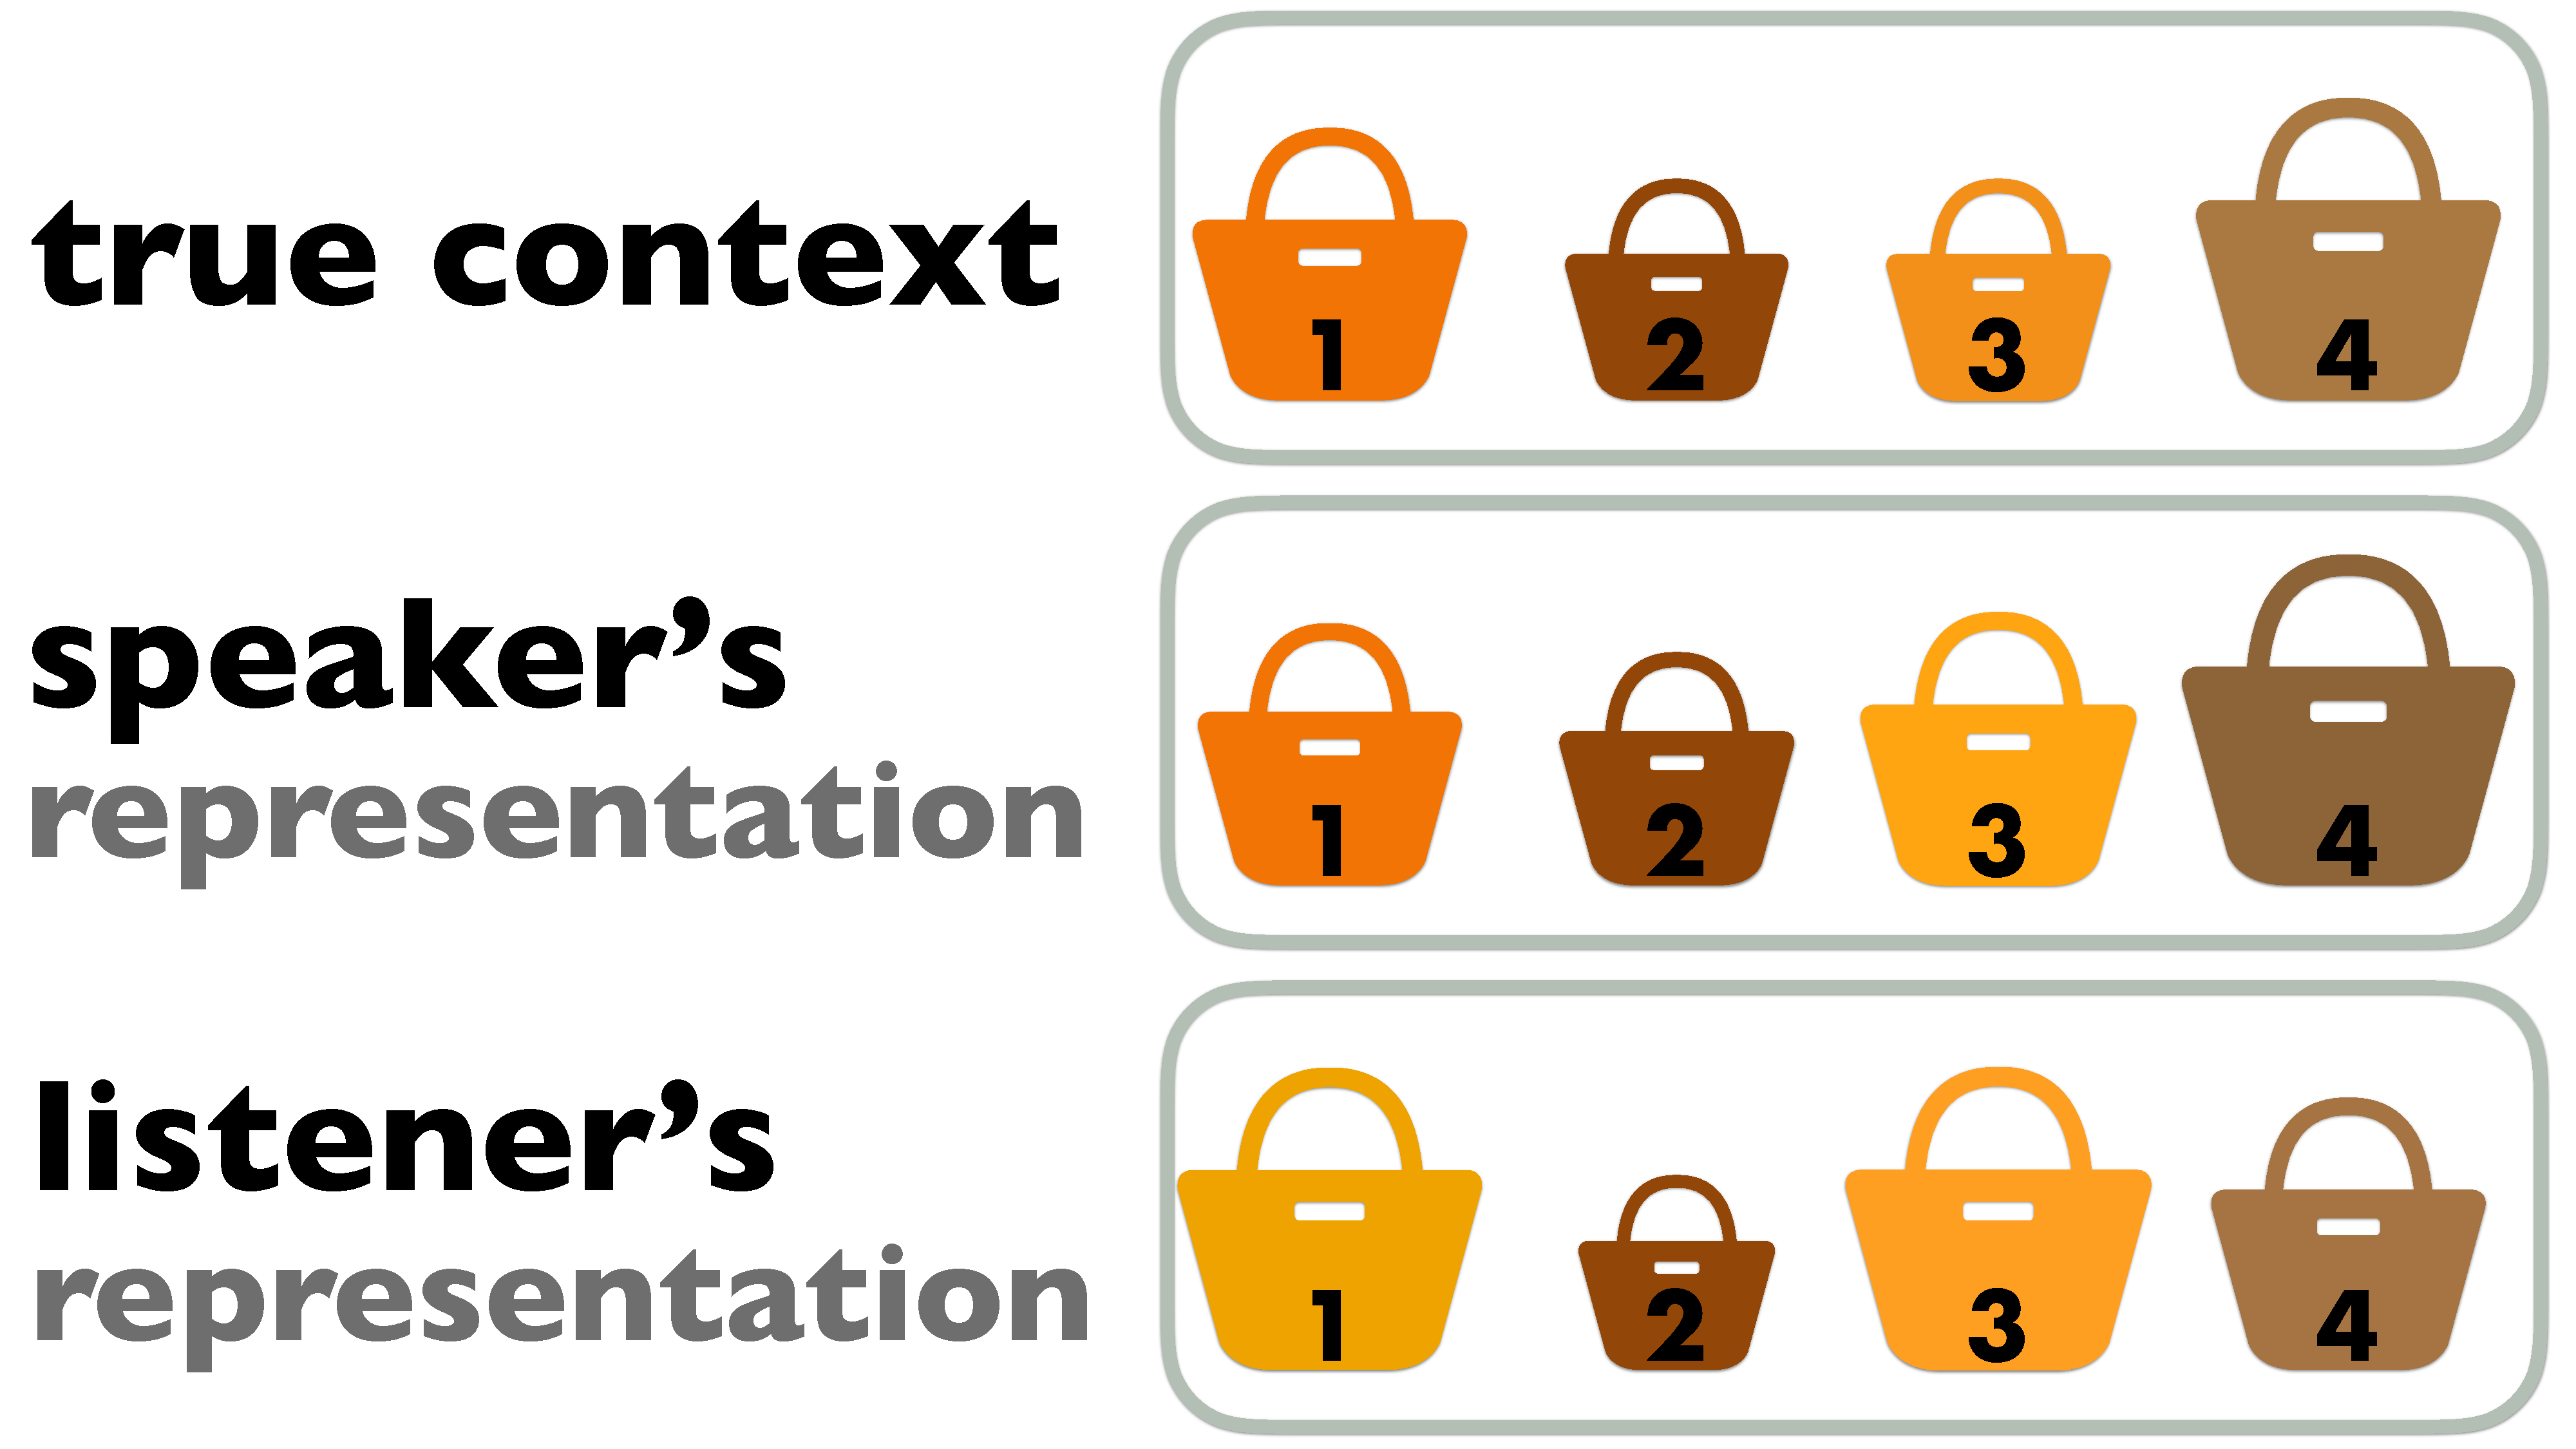
\includegraphics[width=\linewidth]{model_picture.pdf} 
  \caption{Illustration of the model}
  \label{fig:ModelIllustration}
\end{figure}

\bibliographystyle{apacite}
\setlength{\bibleftmargin}{.125in}
\setlength{\bibindent}{-\bibleftmargin}

\bibliography{adjOrder}

\end{document}

